\documentclass[bfvec]{summery_5.0}
\title{Experimentalphysik Va - Zusammenfassung}

\begin{document}
\maketitle
\tableofcontents

\part{Festkörpermodelle}
\section{Modelle der Wärmekapazität}


Auf jeden Freiheitsgrad fällt, wenn er quadratisch in die Hamiltonfunktion eingeht, nach dem Gleichverteilungssatz, auch Äquipartitionstheorem, die kinetische Energie:
\begin{align*}
    \boxed{\te{\bf Gleichverteilungssatz:}\qquad  E\sub{kin} = \frac12 k_B T}
\end{align*}

Man definiert die spezifische Wärmekapazität \(C\) mittels der zugeführten Wärmemenge \(\Delta Q\) als

\begin{empheq}{align*}
    \te{\bf Wärmekapazität:}\qquad C&=\pp UT
\end{empheq}

\subsection{Bose-Einstein Statistik}
Die Besetzungswahrscheinlichkeit eines quantenmechanischen Zustandes \(\ket {E_n}\) ist propotional zum Bolzmann-Faktor:
\begin{align*}
    \boxed{\te{\bf Bolzmannfaktor:} \qquad P_n\propto e^{-\frac{E_n}{k_B T}}}
\end{align*}
Die Normierung ist natürlich von den gegebenen \(E_n\) abhängig. Für den Erwartungswert erhält man mit der Zustandssumme \(Z\equiv \sum_n e^{-\beta E_n}\) als gesamt Gewicht und \(\beta = \frac1{k_B T}\):
\begin{align*}
    \tug E &= \sumii n E_n P_n = - \pp {}\beta \ln Z 
\end{align*} 
Speziell für den harmonischen Oszillator, dessen Energieniveaus 
äquidistant sind, ergibt sich mit \(x \equiv \frac{\hbar\omega}{k_B T}\)
\begin{align*}
    \tug E &= \hbar \omega \hug{\frac12 +\tug n_T}
    = \frac{\sumii n e^{-x (1/2 + n)}\cdot  \hbar\omega (1/2 + n)}{\sumii n e^{-x (1/2 + n)} }
    = \hbar\omega\hug[\Bigg] {\frac12 + \underbrace{\frac{\sumii n e^{-x n}\cdot n}{\sumii n e^{-x n} }}_{\tug n_T}}\\
    \tug{n}_T 
    &= \frac{\sumii n \hug{e^{-x}}^n\cdot n}{\sumii n \hug{e^{-x}}^n }
    = \frac{-\pp{}{x}\sumii n \hug{e^{-x}}^n}{\sumii n \hug{e^{-x}}^n }
    = -\hug{1-e^{-x}}\pp{}{x}\frac1{1-e^{-x}}
    = \frac{1}{e^x-1}\\
\end{align*}

\begin{boxA}
{\bf Bose-Einstein-Statistik für den quantenmechanischen harmonischen Oszillator:}

Die Bose-Einstein Statistik
\begin{align*}
    \tug{n}_T = \frac{1}{e^x-1}, \qquad x\equiv \frac{\hbar\omega }{k_B T}
\end{align*}
ist gültig für Teilchen mit ganzzahligem Spin (Bosonen). Man interpretiert die verschiedenen Oszillator-Moden nicht als tatsächliche Bewegung eines einzelnen Teilchens, sondern als abstrakte
„Quasiteilchen“ - Phononen der Energie $\tug E$, die entsprechend mit der Mode $\omega = E/\hbar$ schwingen. Tatsächlich gilt die Bose-Einstein Statistik allgemein in einer quantenmechanischen Beschreibung eines Gases aus Bosonen.
\end{boxA} 

\subsection{Dulong-Petit-Gesetz}
Für hohe Temperaturen gibt es für die Wärmekapazität von Festkörpers einen universellen Grenzwert. Nach dem Gleichverteilungssatz entfällt auf jeden Freiheitsgrad eine kinetische Energie von $\frac12 k_B T$, und nach dem Virialsatz ist die mittlere kinetische gleich der mittleren potentiellen Energie. Insgesamt also $E = k_B T$ pro Freiheitsgrad, was bei drei Raumdimensionen den Dulong-Petit-Grenzwert ergibt:
\begin{align*}
    \fboxed{Dulong-Petit-Grenzwert}{C = 3k_B }
\end{align*}

Für sehr tiefe Temperaturen findet man empirisch für Metalle den Zusammenhang \(C = aT + bT^3\), für nicht Metalle entfällt der lineare Term. Dies ist nur im Rahmen der Quantenmechanik zu erklären.

\subsection{Einstein Modell}
Einsteins Ziel war es qualitativ zu zeigen, dass eine quantenmechanische Beschreibung der Wärmekapazität nötig ist, um diese im Bereich niedriger Temperaturen zu erklären. Dazu betrachtete er die Gitterschwingungen des Festkörper als Verbund vieler harmonischer Oszillatoren: 
\begin{align*}
    C &= \pp{\tug E}T 
    = \pp{}{T} \hug{\hbar\omega \hug{\frac12+ \tug n_T}} 
    = k_B x^2 \frac{e^x}{(e^x-1)^2}
\end{align*}
In drei Dimensionen ist aufgrund von 
\begin{align*}
    E_{n_x,n_y,n_z} &= \hbar\omega \bug{\hug{n_x+\half} + \hug{n_y+\half} +\hug{n_z+\half}}\\
    Z_{3D} &= \sum_{n_x,n_y,n_z} e^{-\beta E_{n_x,n_y,n_z}}= Z_{1D}^3\\
    \tug{E_{3D}} &= -\pp{}\beta \ln Z_{3_D} = 3 \tug{E_{1D}}
\end{align*} 
die Wärmekapazität einfach das dreifache des eindimensionalen Falls.
\begin{align*}
    \boxed{C = 3k_B x^2 \frac{e^x}{(e^x-1)^2}}
\end{align*}
Für tiefe Temperaturen beschreibt die Relation korrekt ein einfrieren 
der Freiheitsgerade $(C(T=0)=0)$, und für hohe Temperaturen geht es ins Dulong-Petit Gesetz über.
Den einzigen Parameter \(\omega\equiv \omega_E\) in Einsteins Beschreibung der Wärmekapazität, nennt man die Einstein Frequenz.

\subsection{Debye Modell}
Debye verbesserte das Einstein-Modell mit der Annahme, dass die Oszillationen der Atome genau so quantisiert werden müssen, wie es Planck mit den Lichtwellen tat. 
Die einzige Unterschiede sin, dass Schallwellen drei Polarisationsrichtungen haben und die Dispersionsrelation modifiziert werden muss zu $\omega = vk$.\\

{\bf Herleitung:}\\
Um die Wärmekapazität $C = \pp {\tug E}T$ zu bestimmen, wird zunächst $\tug E $ 
bestimmt. Es gilt:
\begin{align*}
    \tug E &= \int_0^{E_D}\d E g(E)\tug n E 
\end{align*}
Wobei $\tug n$, die Besetzungszahl, einer Bose-Verteilung entspricht, da es sich bei Phononen um Bosonen handelt. 
Um die Zustandsdichte $g(E)$ zu berechnen muss man sich als erstes die Quantisierung überlegen:
\begin{align*}
    L &= n \frac{\lambda}{2} \Leftrightarrow k = \frac{n\pi}{L}
\end{align*}
Die Zustandsdichte ist dann als Funktion von $k$, bzw. von $E$ mit $g(k)\dk = g(E)\d E$: 
\begin{align*}
    g(k)\dk  &= \underbrace{3}\sub{Polarisation}\cdot \underbrace{\hug{\frac{L}{\pi}}^3}\sub{Moden pro Vol.} \cdot \underbrace{\frac{4\pi k^2}{8}\dk}\sub{Vol. im k-Raum}\quad  \Leftrightarrow\quad  g(E) = \frac{3}{2\pi^2}\frac{V}{\hbar^3 c^3} E^2
\end{align*}
Es können mikroskopisch maximal $3N$ Moden existieren, sodass es eine höhste anregbare Energie gibt, die sog. \emph{Debye-Energie} $E_D$:
\begin{align*}
    3N \peq \int_0^{E_D} \d E g(E) = \frac{V}{2\pi^2 \hbar^3 c^3} E_D^3 \quad\Leftrightarrow\quad E_D^3 = \frac{6\pi^2 N \hbar^3 c^3}{V}
\end{align*}

Alle benötigten Größen sind nun berechnet und die Wärmekapazität ergibt sich als:
\begin{align*}
    \Aboxed{C &= 9N k_B \frac{T^3}{T_D^3}\int_0^{T_D/T} \d x \frac{x^4 e^x}{(e^{x} -1)^2}}
\end{align*}
Das Integral ist nicht analytisch Lösbar, aber für niedrige Temperaturen kann man die obere Grenze des Integral gegen unendlich gehen lassen, und man erhält das gewünschte \(T^3\) Gesetz:
\begin{align*}
    \boxed{C(T\ll T_D)= \frac{12\pi^4}{5} N k_B \hug{\frac T{T_D}}^3}
\end{align*}
Für hohe Temperaturen geht das Integral in dne Dulong-Petit Grenzwert $C=3N k_B$ über. Das Debye-Modell beschreibt die Wärmekapazität richtig im Bereich von niedrigen und hohen Temperaturen, hat aber Abweichungen dazwischen, weil nur akustische Moden berücksichtigt werden. 


\section{Elektronen in Metallen}
Bekannter maßen gibt es in er Wärmekapazität von Metallen, einen linearen Term $C(T) = \gamma T + \beta T^3$. Um diesen zu erklären, müssen die Elektronen im Material berücksichtigt werden. 

\subsection{Drude Modell}
Das Drude Modell ist eine klassische Beschreibung.
\begin{boxA}
{\bf Annahmen im Drude Modell:}
\begin{itemize}
    \item Die Leitungselektronen im Metall erfahren durch die Atomrümpfe im Mittel nur ein effektives Kastenpotential und wechselwirken miteinander bis auf Stöße nicht. Sie verhalten sich wie ein \emph{ideales Gas}.
    \item Daher folgen sie der \emph{Maxwell-Boltzmann-Verteilung} mit einer mittleren Geschwindikeit von 
    \begin{align*}
        \tug v &= \sqrt{\frac{8 k_B T}{\pi m_e}}
    \end{align*}
    \item Elektronen unterliegen im Metall Steuprozessen, wobei die mittlere Zeit zwischen zwei Streuprozessen, die sog. \emph{Relaxionszeit} $\tau$ ist. Sie ist für feste Temperaturen konstant. 
    \item Nach einem Streuprozess besitzt besitzt ein Elektron statistisch den Impuls $\v p = 0$.
    \item Zwischen den Streuprozessen reagieren die Elektronen aufgrund ihrere Ladung auf äußere elektromagnetische Felder.
\end{itemize}
\end{boxA}

Betrachten wir die zeitliche Entwicklung des Impulses als gewichteten Mittelwert:
\begin{align*}
    \v p (t+\dt) &= \underbrace{\v 0 \cdot \frac{\dt}\tau}\sub{Stoß} + \underbrace{(\v p + \v F \dt )\hug{1-\frac{\dt}\tau}}\sub{kein Stoß}\\
    \v p + \dd{\v p}t \dt&= \v p + \hug{\v F-\frac{\v p}\tau} \dt \\ 
   \Aboxed{ \dd{\v p}t &= \v F-\frac{\v p}{\tau}  }
\end{align*}
Es stellt sich somit bei einer konstanten Kraft ein Gleichgewicht ein.

\subsubsection{Elektrische Leitfähigkeit}
Nehmen wir nun an, dass die Kraft durch ein E-Feld vermittelt wird, und sich ein Gleichgewicht $\dotv p  = 0$ angenommen hat. Dann gilt nach der letzten Formel für die Drift-Geschwindigkeit der Teilchen:
\begin{align*}
    v &= \mu E ,\qquad \mu = \frac{q\tau}{m_e}
\end{align*} 
mit der sog. Mobilität $\mu$.
Mit der Stromdichte $j = \rho v = -nev$ (Teilchendichte $n$) erhält man aus diesen Rechnungen eine Beziehung zwischen Leitfähigkeit und Relaxationszeit, sowie die mikroskopische Form des ohmschen Gesetztes:
\begin{align*}
    \fboxed{Drude Formel}{j=\sigma E, \qquad \sigma=\frac{ne^2}{m_e}\tau}
\end{align*}
mit der Leitfähigkeit $\sigma$.

\subsubsection{Wärmeleitung}
Die Wärmeleitung wird durch das Fourier-Gesetz beschrieben (Wärmeleitfähigkeit $\kappa$):
\begin{align*}
    \v j_Q &= -\kappa \grad T,\qquad \kappa = \frac{n c_V \tug v^2\tau}{3}
\end{align*}
Da die Elektronen als ideales Gas beschrieben werden gilt:
\begin{align*}
    c_V = \frac f2 k_B= \frac32 k_B, \qquad \tug v &= \frac{8 k_B T}{\pi m}
\end{align*}
Dadurch erhält man unter der Annahme, dass thermische und elektrische Relaxionszeiten gleich sind:
\begin{align*}
    \fboxed{Wiedemann-Franz-Gesetz}{\frac\kappa\sigma = \frac{4 k_B^2}{\pi e^2}T}
\end{align*}
Der Quotient der thermischen und elektrische Leitfähigkeit ist also materialunabhängig. Man definiert in diesem Kontext noch die sog. Lorenz-Zahl:
\begin{align*}
    L = \frac{\kappa}{\sigma} T
\end{align*}

\subsubsection{Probleme mit dem Drude-Modell}
Die erhaltenen Lorenz-Zahlen sind prinzipiell zu klein. Tatsächlich ergibt sich die Lorenz-Zahl überhaupt nur durch Zufall in der korrekten Größenordnungen! Eigentlich führen die Annahmen des Drude Modelles auf zwei sehr große Fehler:
\begin{enumerate}
    \item Die klassische Wärmekapazität $C=\frac32 Nk_B$ ist etwa um einen Faktor 100 zu groß.
    \item Die klassische mittlere Geschwindigkeit $\frac12m_e v^2 = \frac32 k_B T$ ist stark unterschätzt, ebenfalls etwa um einen Faktor 100.
\end{enumerate}
Außerdem sieht man bereits, dass das Drude Modell die gefundene $\propto T$ Abhängigkeit der Wärmekapazität nicht beschreiben kann.

Um die Fehler des Drude Modells zu überprüfen kann man auch den sog. Peltier-Effekt verwenden. Dieser beschreibt das Entstehen eines Wärmestroms aufgrund eines anliegenden elektrischen Feldes. Der umgekehrte Effekt heißt Seebeck-Effekt. In dem hierbei erhaltenen Quotient aus elektrischem und thermischen Strom kompensieren sich die beiden Fehleranteile nämlich nicht, sodass man ein um zwei Größenordnungen falsches Ergebnis erhält

\subsection{Sommerfeld Modell}
Das Sommerfeld Modell ist eine quantenmechanische Beschreibung.
\begin{boxA}
    {\bf Annahmen im Sommerfeld-Modell:}
    \begin{itemize}
        \item Die Leitungselektronen im Metall erfahren durch die Atomrümpfe im Mittel nur ein effektives Kastenpotential. Sie liegen delokalisiert im Metall vor.
        \item Die Wechselwirkung der Valenzelektronen untereinander wird vernachlässigt.
        \item Die Elektron verhalten sich wie ein Fermi-Gas und folgen somit der Fermi-Dirac-Verteilung.
    \end{itemize}
\end{boxA}

\subsubsection{Zustandsdichte und Fermi-Größen}
Wir betrachten das Metall als Potentialtopf und suchen die Lösungen der Schrödingergleichung. Periodische Randbedingungen führen zu Ebenen Wellen, mit quantisierten Wellenvektoren
\begin{align*}
    \v k =\frac{\pi}{L} \v n 
\end{align*}

Unter Berücksichtigung der Spin Entwartung $g_s=2$ und der Dispersionsrelation $E = \frac{(\hbar k)^2}{2m}$ ergibt sich die Zustandsdichte als:
\begin{align*}
    \Aboxed{\te{\bf Zustandsdichte:}\quad g(k) &= g_s \frac18 \hug{\frac L\pi}^3 4\pi k^2\quad \Leftrightarrow \quad 
    g(E) = \frac{\sqrt 2}{\pi^2}\frac{V m^\frac32}{\hbar^3} \sqrt E}
\end{align*}

Für niedrigere Energien können aufgrund des Pauliprinzips nicht alle Elektronen in den niedrigsten Energiezustand kondensieren. Stattdessen werden die niedrigsten Energienivaus der Reihe nach aufgefüllt. Man nennt die Grenzenergie zwischen besetzten und unbesetzen Niveaus Fermi-Energie $E_F$:
\begin{align*}
    \Aboxed{\te{\bf Fermi-Energie:}\quad N &= \int_0^{E_F} \d E g(E)\quad \Leftrightarrow\quad E_F =\frac{\hbar^2}{2m}\hug{\frac{3\pi^2 N}{V}}^\frac23}
\end{align*}
An dieser Stelle führt man einige von der Fermi-Energie abgeleiteten Größen ein:
\begin{empheq}{align*}
    k_F &= (3\pi^2 n)^{\frac13} \qquad  v_F = \frac{\hbar k_F}{m_e}\\
    E_F &= \frac{\hbar^2 k_F^2}{2m_e} \quad\qquad T_F = \frac{E_F}{k_B}
\end{empheq}

\subsection{Beitrag zur Wärmedichte}
Für niedrige Temperaturen entwickelt man die Fermi-Dirac Verteilung, und erhält die sog. Sommerfeldentwicklung:
\begin{align*}
    C = \frac{\pi^2}{2}Nk \frac T {T_F} + \bigO{\frac{T}{T_F}}^3
\end{align*}
Dies liefert das korrekte $\propto T$ verhalten, welches in der Drude-Theorie fehlt. Man kann die Drude Gleichung als die Bewegung des Schwerpunktes der Fermikugel interpretiert.

\section{Chemische Bindungen}
\begin{itemize}
    \item {\bf Ionische Bindung:} Elektron geht komplett von einem Bindungspartner auf das andere über. Wird quantitativ gut beschrieben durch das Born-Mayer-Potential: $U(r) = 2Be^{-r/\rho}-\frac{e^2}{4\pi\epsilon_0 r}\alpha $, mit dem materialspezifischen Konstanten $\alpha, B$. Die Bindungsenergien liegen in einem Bereich von etwa $E\in[5,10]\u {eV}$.
    \item {\bf Kovalente Bindung:} Eine oder mehere Elektronen bilden ein sog. bindenes Orbital, welches sich über beide Bindungspartner erstreckt. Dadruch wird die Delokalisierung der Elektronen größer und es ergibt sich ein energetisch günstigerer Zustand. Der erste Angeregte Zustand heißt antibindenes Orbital kann im Fall von z.B. Helium dafür sorgen, dass es zu keiner Bindung kommt, da die Elektronen sowohl das bindene als auch antibindene Orbital besetzten müssen, wodurch sich die Energie insgesamt nicht senkt. Die Bindungsenergien liegen in einem Bereich von etwa $E\in [5,10]\u{eV}$.
    \item {\bf Metallische Bindung:} Die hohe Delokalisierung der Elektronen führt ähnlich zur kovalenten Bindung zu einem Energievorteil. Die Bindungsenergien liegen in einem Bereich von etwa $E\sim1\u{eV}$.
    \item {\bf Hybridisierung:} Überlagerung von allen Bindungstypen. 
    \item {\bf Van-Der-Waals-Bindung:} Entsteht durch Dipolmomente, welche durch zufällige Quantenfluktuationen hervorgerufen werden, und weitere Dipol induzieren. Wird beschrieben durch das Lennard-Jones-Potential: $U(r) = 4\epsilon\bug{\hug{\frac \sigma R}^{12} - \hug{\frac{\sigma}{R}}^6}$, wobei der $R^{-12}$-Term die Abstoßung durch das Pauliprinzip modeliert. Das Potenzial ist so parametrisiert, dass $U(\sigma)=0$ und $\min U(r) = U\hug[\big]{\sqrt[6]2\sigma }= -\epsilon$. Die Bindungsenergien liegen in einem Bereich von etwa $E\in [0.05, 0.1]\u{eV}$.
\end{itemize}

\subsection{Materialklassen}
Man quantisiert die Ordnung von Materialien mit der Paarkorrelationsfunktion $g(\v r_1, \v r_2) = \frac{1}{n_0^2} \tug{n(\v r_1)n(\v r_2)}$
\begin{itemize}
    \item {\bf Kristalle:} periodisch angeordneter Verbund von Atomen, deterministische Fernordnung
    \item {\bf Flüssigkeit:} Nahordnung aber keine Fernordnung, mobile Atome
    \item {\bf Gas:} Keine Ordnung, raumfüllend.
    \item {\bf Flüssigkristall:} kristalline Ordnung nur in einer Raumrichtung.
    \item {\bf Quasikristalle:} deterministische Fernordnung, aber keine periodische Struktur. In einer Dimension realisierbar durch aperiodische Multilayer, z.B. mit der Fibonacci-Folge.
    \item {\bf Polymere:} bestehen aus sehr langen Ketten von Atomen.
\end{itemize}

\section{Festkörpermodelle in 1D}
\subsection{Kompressibilität, Schall und thermische Ausdehnung in 1D}
{\bf Kompressibilität}

Die Taylorentwicklung eines Wechselwirkungspotentials um den Gleichgewichtspunkt ist:
\begin{align*}
        V(x) &= \underbrace{V(x_0) + \frac{D_2}{2}(x-x_0)^2}\sub{harmonisch} + \underbrace{\frac{D_3}{3!}(x-x_0)^3 + \dots}\sub{anharmonisch}
\end{align*}
Wir definieren die \emph{Kompressibilität} $\beta$ und das \emph{Kompressionsmodul} $K$ durch
\begin{align*}
        \Aboxed{\beta &=\frac 1K= -\frac{1}{V}\pp Vp\eval_{T/S} \sim-\frac{\Delta V/V}{\Delta p}}
\end{align*}
In einem eindimensionalen Modell mit $S=T=0$ wird der Druck zu einer Kraft, und das Volumen zu einer Länge:
\begin{align*}
    \beta\sub{1D} &= -\frac1L \pp LF\eval_{L=L\sub{eq}}
\end{align*}
In harmonischer Näherung gilt dann nach dem Hookschen Gesetz:
\begin{align*}
    \Aboxed{\beta=-\frac1{Da}}
\end{align*}
mit dem Gleichgewichtsabstand zwischen zwei Nachbarn $a$.

\subsubsection*{Schall}
Die Ausbreitung von mechanischen Wellen benötig eine \emph{Trägheitseigenschaft} und eine \emph{elastische Eigenschaft}.
Die Schallgeschwindigkeit ist in verschiedenen Materialien grundsätzlich der Form 
\begin{align*}
    v= \sqrt{\frac{\te{elastische Eigenschaft}}{\te{Trägheitseigenschaft}}}
\end{align*}
Es ergebenen sich in verschiedenen Umständen die folgenden Schallgeschwindigkeiten:
\begin{itemize}
    \item gespannte Saite: $v=\sqrt{\frac F{\rho\sub{lin}}}$
    \item Fluide: $v=\sqrt {\frac K\rho} =\sqrt{\frac {1}{\beta \rho}}$
    \item Ideales Gas: $v=\sqrt{\frac{\gamma k_B T}{m}}$, mit $\gamma=c_p/c_V$ als Adiabaten-Koeff. 
    \item 1D-Kristall: $v = \sqrt{\frac{Da^2}{m}}$ 
    \item elastischer Stab (Festkörper): $v = \sqrt{\frac E\rho}$, mit dem Elastizitätsmodul $E= \frac{\Delta F/A}{\Delta l/l}$
\end{itemize}

\subsubsection*{Thermische Ausdehnung}
Die Ausdehnung eines Materials bei einer Erhöhung Temperatur entsteht durch die Anharmonizität des Potenzials. Das Potenzial wird also asymmetrisch um den Gleichgewichtsabstand, und es werden durch die thermische Energie mehr Zustande mit größerem als kleineren Abstand angeregt. Im klassischen Fall berechnet man den erwarteten Abstand im kanonischen Ensemble als:
\begin{align*}
    \tug x_T = \frac{\int \dx x e^{-\frac{U(x)}{k_B T}}}{\int \dx e^{-\frac{U(x)}{k_B T}}}
\end{align*}
Da bereits der erste anharmonische Term des Potential nicht mehr integrierbar ist macht man folgenden Näherung:
\begin{align*}
    e^{-\beta U} &\approx e^{-\beta\hug{\frac{D_2}{2}(x-x_0)^2 + \frac{D_3}{3!}(x-x_0)^3}} \approx e^{-\beta\frac{D_2}{2}(x-x_0)^2}\hug{1-\frac{D_3}{3!k_B T}(x-x_0)^3}
\end{align*}
Dann ergibt sich mit dem Ausdehnungskoeffizienten $\alpha$:
\begin{align*}
    l = l_0 (1+\alpha \Delta T)
\end{align*}


\subsection{Monoatomare lineare Kette}
Wir betrachten eine eindimensionale lineare Kette von Atomen, die in harmonischer Näherung mit der Federkonstanten $D$ an ihren Nachbarn koppeln.
Das Potenzial lautet also 
\begin{align*}
    V\sub{ges} &= \sum_n \frac12 D(\delta x_{n+1}-\delta x_n)^2\\
    F_n &= m\delta \ddot x_n = -\pp {V\sub{ges}}{\delta x_n} = D(\delta x_{n+1} -2\delta x_n + \delta x_{n-1})
\end{align*}

Die Lösungen der Bewegungsgleichung sind die ebene Wellen mit diskretem Träger:
\begin{align*}
    \delta x_n &= A\exp(i(\omega t- kna))
\end{align*}

Einsetzen in die Bewegungsgleichung liefert eine periodische Dispersionsrelation:
\begin{align*}
    \Aboxed{\omega &= 2\sqrt{\frac Dm} \abs{\sin\hug{\frac{ka}{2}}}}
\end{align*}

Die Schallgeschwindigkeit ist
\begin{align*}
    c_s &= \pp\omega k 
    = a\sqrt{\frac Dm} \cos\hug{\frac{ka}{2}}
    \approx \begin{cases}
        a \sqrt{\frac Dm}\for k\approx  0\\
        0 \for k \approx \frac {\pi} a
    \end{cases}
\end{align*}
Für kleine Wellenzahlen $k$ ist die Dispersion ungefährt linear, dieser Bereich beschreibt Schallwellen im Debye-Modell. Es gibt auch Bereiche in denen es zu stehenden Wellen kommt ($\pp\omega k =0$), die durch Bragg-Reflexion entstehen.

Die Zustandsdichten können aus der periodischen Randbedingung $\delta x_n = \delta_{x+N} \Leftrightarrow k = m \frac{2\pi}{L}$ berechnet werden als:
\begin{align*}
    g(k) &= \frac{Na }{2\pi} \\
    g(\omega) &= 2 g(k) \dd k \omega = \frac{2N}{\pi}\frac1{\sqrt{\omega\sub{max}^2 - \omega^2}}
\end{align*}

\subsubsection{Reziprokes Gitter}
Ist die Struktur im Ortsraum periodisch mit Periode $a$, so ist die Dispersionrelation im $k$-Raum periodisch mit Periode $2\pi/a$. Die Einheitszelle im $k$-Raum nennt man die 1. Brillouinzone. Man nennt die Atome selbst auch direktes Gitter, und das $k$-Gitter auch reziprokes Gitter.

\subsection{Phononen}
Phononen sind die Quanten der Gitterschwingungen. Ihre Eigenschaften sind:
\begin{itemize}
    \item Träger von Energie $\hbar\omega$, Impuls $\hbar k \mod \hbar G_n$ ($G_n = n\frac{2\pi}{a}$ es wird also immer der Impuls aus der ersten Brillouinzone verwendet\footnote{Dies widerspricht nicht den Erhaltungssätzen, da die Impulserhaltung nach dem Noether Theorem auf einer \emph{kontinuierlichen} Translationssymmetrie beruht, die hier nicht vorliegt.}) und eines Drehimpules
    \item Mehrfachbesetzungen desselben Zustandes möglich $\to$ Bosonen 
    \item Anzahl der Zustände in der 1. Brillouinzone = $N$
\end{itemize}



\subsection{Zweiatomige lineare Kette}
Wir betrachten nun eine lineare Kette aus zwei sich abwechselden Teilchenarten $x$ und $y$ mit Masse $m$. Auch die Federkonstante soll sich abwechseln zwischen $D_1$ und $D_2$. Die Kraftgleichungen sind dann
\begin{align*}
    m \delta \ddot x_n &= F_n^x = D_2 (\delta y_n - \delta x_n) + D_1(\delta y_{n-1} -\delta x_n)\\
    m \delta \ddot y_n &= F_n^y = D_1 (\delta x_{n+1} - \delta y_n) + D_2(\delta x_{n} -\delta _n)
\end{align*}
Wir machen für $\delta x$ und $\delta y$ wieder den Ansatz ebener Wellen mit diskretem Träger.
\begin{align*}
    \delta x_n= A_x e^{i(\omega t - kna)},\qquad
    \delta y_n= A_y e^{i(\omega t - kna)}
\end{align*}
Dadurch erhält man: 
\begin{align*}
    m\omega^2 \binom{A_x}{A_y} = \m{D_1+D_2& -D_2 - D_1 e^{ika}\\ -D_2 - D_1 e^{-ika} & D_1 + D_2} \binom{A_x }{A_y}
\end{align*}
Dies ist ein Eigenwertproblem der Matrix. Die Existenz zweier linear unabhängiger Eigenvektoren/-werten ist durch die Selbstadjungiertheit garantiert. Die Eigenwerte ergeben die Dispersionsrelation:
\begin{align*}
    \Aboxed{\omega_\pm^2 &= \frac{D_1+D_2}{m} \pm \frac1{m}\sqrt{D_1^2 + D_2^2 + 2D_1D_2 \cos(ka)}}
\end{align*} 
Es gibt zwei reelle $\omega$-Werte für jedes $k$. Die Lösung $\omega_+$ bezeichnet man als \emph{optischen Zweig}, es handelt sich um gegenphasige Schwingungen benachbarter Atome, weshalb diese Moden nicht durch Schall sondern haubtsächlich durch optische Neutronen/Protonen oder Röntgen-Synchrotronstrahlung angeregt werden. Die $\omega_-$-Lösung bezeichnet man als \emph{akustischen Zweig}, hier Schwingen die Atome in Phase. 

\begin{figure}[H]
    \centering
    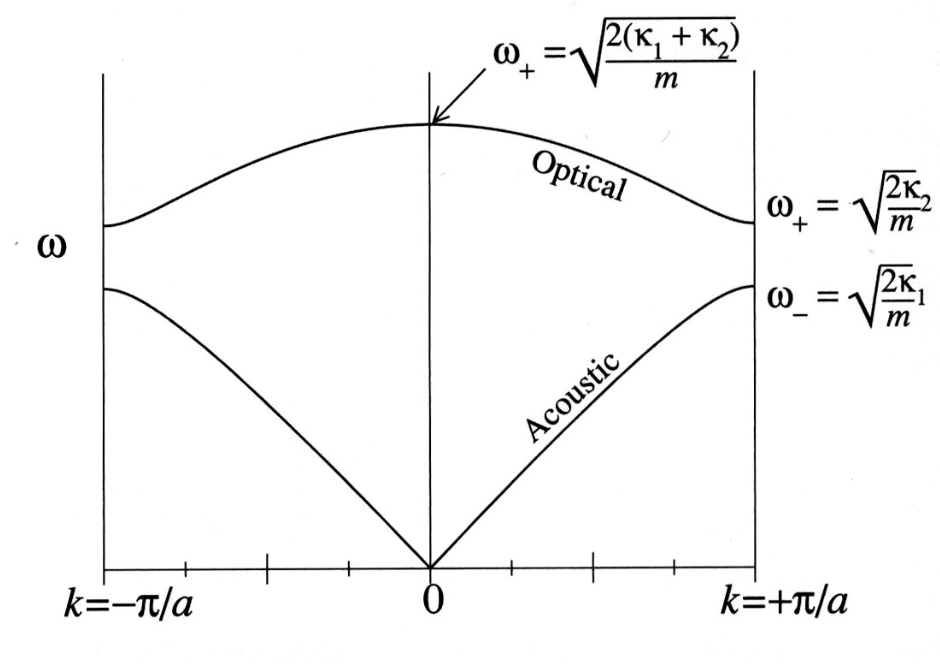
\includegraphics[width=.6\textwidth]{zweige.png}
    \caption{Dispersionskurve der Diatomaren linearen Kette. Eine Animation der zugehörigen Gitterschwingungen findet sich \href{file:./Diatomic_chain.gif}{hier}.}
\end{figure}

% \begin{figure}[H]
%     \centering
%     \includegif[width=1.0\textwidth]{Diatomic_chain.gif}
%     \caption{Vibrationen des Gitter zu verschiedene Frequenzen und Wellenzahlen}
% \end{figure}


\subsection{Verallgemeinerung: M-atomige lineare Kette}
\begin{table}[H]
\centering
\begin{tabular}{@{}llll@{}}
    \toprule
    & \multicolumn{3}{c}{Kette} \\\cmidrule(lr){2-4}
    &einatomig & zweiatomig & $M$-atomige Kette \\
    \midrule
    Einheitszellen & $N$ & $N$ & $N$ \\
    Atome & $N$ & $2N$ & $MN$ \\
    Moden & $N$ & $2N$ & $MN$ \\
    Zweige & $1$ & 2 & $M$ \\
    (akustisch) & 1 & 1 & 1 \\
    (optisch) & 0 & 1 & $M-1$ \\
    \bottomrule
\end{tabular}
\end{table}

\section{Magnetismus}
Die magnetische Suszeptibilität $\chi$ beschreibt die Reaktion eines Materials auf ein äußeres Magnetfeld:
\begin{align*}
    \v M = \chi \v H
\end{align*}
Es gibt gibt verschiedene Typen von magnetischen Materialien, abhängig von dem Wert von $\chi$:
\begin{itemize}
    \item {\bf Diamagnetismus:} $\chi<0$, die induzierten Dipole zeigen entgegen das angelegten H-Feld, sodass die potentielle Energie $U=-\v \mu\cdot\v B $ steigt. Das Material wird daher aus dem Feld herausgedrückt.
    \item {\bf Paramagnetismus:} $\chi>0$, die induzierten Dipole zeigen parallel zum angelegten Feld, die potentielle Energie sinkt also, sodass das Material in das Feld reingezogen wird. 
    \item {\bf Ferromagnetismus:} $\chi\gg0$, ähnlich wie der Paramagnetismus, jedoch sind die Wechselwirkungen unter dn magnetischen Momenten im Material so stark, dass sie sich auch ohne externes B-Feld parallel ausrichten. Das Material ist also permanent magnetisch.  
\end{itemize}

\subsection{Pauli-Paramagnetismus}
Der Pauli-Paramagnetismus beschreibt den Paramagnetismus so, dass sich durch anlegen eines B-Feldes die Energieniveaus der Elektronen, je nach Spin, nach dem Prinzip des Zeemann-Effekts verschieben:
\begin{align*}
    \Delta E = \pm \mu_B B
\end{align*} 
Es kommt so zu einer Verschiebung der Fermikante und Elektronen besetzten zu einem gewissen Anteil preferiert Energieniveaus mit parallelen Spins. Für kleine Temperaturen erhält man:  
\begin{align*}
    \Aboxed{\te{\bf Pauli-Suszeptibilität:}\quad \chi=\frac{3N\mu\mu_B^2}{2 E_F} \bug{1- \frac{\pi^2}{12}\hug{\frac T{T_F}^2}}}
\end{align*}

\subsection{Supraleitung}

\part{Kristalle }
\section{Kristallgitter}
\subsection{Definition}
\begin{boxA}
{\bf Gitter:} Ein Gitter ist ein unendlich ausgedehnter Satz von Punkten, die sich als ganzzahlige linear Kombination von Basisvektoren ergeben:
\begin{align*}
    R\sub{N-dim} &= \pug{\sum_{i=1}^N n_i \v a_i : n_i \in \Z, \v a_i \in \R^N}
\end{align*} 
\end{boxA}

\subsection{Begrifflichkeiten}
\begin{itemize}
    \item {\bf Basis:} Positionsangabe der Atome in einer Einheitszelle relativ zum Gitterpunkt.
    \item {\bf Einheitszelle:} Räumlicher Bereich, der in alle Raumrichtungen identisch (periodisch) wiederholt wird und dabei den gesamten Raum ausfüllt.
    \item {\bf Primitive Einheitszelle (PEZ):} Eine Einheitszelle, mit nur einem enthaltenen Gitterpunkt.
    \item {\bf Wigner-Seitz-Zelle:} Volumen das alle Punkte einhält, die näher am Gitterpunkt liegen als benachbarten Gitterpunkten.
    \item {\bf Konventionelle Einheitszelle:} EInheitszelle, die mehr als einen Gitterpunkt enthält.
    \item {\bf Packungsdichte} $= \frac{\te{Volumen der Atome in EZ}}{\te{Volumen der EZ}}$
\end{itemize}

\subsection{Zentrierung}
Unter Umständen ist nicht praktisch eine primitive Einheitszelle zu wählen, bzw. die primitive Einheitszelle spiegelt nicht alle Symmetrien des Gitter wieder. Z.B. kann das kann man für das rhomboedrische Gitter mit $a=b=c$ und $\alpha=\beta=\gamma\sim109.5^\circ$ eine kubische konventionelle Zelle finden, welche offensichtlich mehr Symmetrien wiederspiegelt, man kathegoriesiert das genannte Gitter daher als kubisch ein (es handelt sich um das bcc Gitter). Man gibt dann zusätzlich zur konventionellen Zelle höhster Symmetrie die \emph{Zentrierung} an. Es gibt die folgenden vier Zentrierungen:
\begin{itemize}
    \item Primitiv (\emph{sc/simple}), ohne zusächliche Punkte
    \item Raumzentriert (\emph{bc/body centered}), ein zusätzlicher Punkt im Zentrum 
    \item Flächenzentiert (\emph{fc/face centered}), zusächliche Punkte im Zentrum aller Flächen
    \item Basiszentriert (\emph{base-centered}) zusächliche Punkte im Zentrum von zwei gegenüberliegenden Flächen 
\end{itemize}
Alle Kristallsysteme mit Zentrierung sind auch ein Gitter, im Sinne von Definition 6.1.

\subsection{Bravaisgitter}
Die Frage, wie viele mögliche Gitter es gibt ist komplex, und wird mithilfe der Gruppentheorie im Detail behandelt. Beschreibt man eine Einheitszelle mittels 3 Basisvektoren der Längen $a,b,c$ sowie drei Winkeln $\alpha,\beta$ und $\gamma$, so erhält man 7 mögliche Achsensysteme. Berücksichtigt man nun noch die Zentrierung erhält man unter Ausschluss von Doppelzählungen 14 sog. Bravaisgitter-Typen.

\begin{table}[H]
\centering
\begin{tabular}{@{}llll@{}}
    \toprule
    Basisvektoren & Winkel & Kristallsystem & mögl. Zentrierungen \\
    \midrule
    $a\neq b\neq c$ & $\alpha\neq\beta\neq\gamma \neq 90^\circ$ & triklin & \hfill-\hspace*{\fill}\\\hdashline
    $a\neq b\neq c$ & $\alpha=\gamma= 90^\circ, \beta \neq 90^\circ$ & monoklin & primitiv, basiszentriert\\\hdashline
    $a\neq b\neq c$ & $\alpha=\beta=\gamma=90^\circ$ & orthorhombisch & primitiv, basiszentriert, \\
    &&&flächenzentriert raumzentriert\\\hdashline
    $a= b\neq c$ & $\alpha=\beta =\gamma= 90^\circ$ & tetragonal & primitiv, raumzentriert\\\hdashline
    $a= b\neq c$ & $\alpha=\beta=90^\circ, \gamma= 120^\circ$ & hexagonal & \hfill-\hspace*{\fill}\\\hdashline
    $a= b= c$ & $\alpha=\beta=\gamma\neq 90^\circ$ & rhomboedrisch & \hfill-\hspace*{\fill}\\\hdashline
    $a= b= c$ & $\alpha=\beta=\gamma= 90^\circ$ & kubisch & primitiv, raumzentriert\\
    &&&flächenzentriert\\
    \bottomrule
\end{tabular}
\end{table}

\subsection{Kugelpackungen}
Echte Kristalle sind nur sehr selten sc (simple cubic). fcc und bcc Strukturen werden in der Natur deutlich häufiger realisiert. Um das zu verstehen kann man sich die Atome als kleine Kugeln vorstellen die sich schwach anziehen und sich daher so dicht wie möglich anordnen. Eine höhere Packungsdichte ist in der Regel energetisch günstiger. Die dichtesten Kugelpackungen sind fcc/face centered cubic und hcp/hexagonal compact packing

\begin{table}[H]
\centering
\begin{tabular}{@{}ll@{}}
    \toprule
    Gitter & Packungsdichte \\
    \midrule
    fcc & $\frac{\pi \sqrt 2}{6}\approx0.74$\\
    hcp & $\frac{\pi \sqrt 2}{6}\approx0.74$\\
    bcc & $\frac{\pi \sqrt3}{8}\approx0.68$\\
    sc & $\frac{\pi}{6}\approx0.52$\\
    \bottomrule
\end{tabular}
\end{table}

\subsection{Rechtwinklige Kristallstrukturen}
Für die häufigsten Bravaisgitter gibt es besondere Bezeichnungen:
\begin{itemize}
    \item Kubisch Flächenzentriert: fcc (\emph{face centered cubic})
    \item Kubisch Raumzentriert: bcc (\emph{body centered cubic})
    \item Primitiv: sc (\emph{simple cubic})
    \item Hexagonal dichteste Kugelpackung: hcp (\emph{hexagonal close-packed})
\end{itemize}

\subsection{Reziprokes Gitter}
\begin{boxA}
{\bf Definition:} Das reziproke Gitter $R$ ist definiert als:
\begin{align*}
    R: \pug{\vec b\in\R^3: \quad e^{i \vec b \vec a} = 1 \ \forall \quad \vec a\in G}
\end{align*} 
Etwas mathematischer kann man es auch als Fouriertransformierte des Gitters auffassen. 
\end{boxA}

Seien die Basis $\vec a_i$ von einem Gitter $G$ und dessen reziprokes Gitter $R$ mit der Basis $b_i$ gegeben. Dann gelten die folgenden nützlichen Identitäten
\begin{align*}
    \Aboxed{\vec b_i = \frac{2\pi}{V\sub{PEZ}}\vec a_j\times \vec a_k, \qquad \vec a_i \cdot \vec b_j = 2\pi \delta_{ij}}
\end{align*}

Es ist nützlich zu wissen, was das reziproke Gitter einer sc/fcc/bcc/hcp Konfiguration ist: $sc\to sc$, $fcc\to bcc$, $bcc \to fcc$, $hcp\to hcp$.

\subsection{Netzebenen und Millerindizes} 
Eine Netzebene enthält mindestens drei linear unabhängige und damit unendlich viele Gitterpunkte. Eine Familie von Netzebenen ist eine unendliche Menge von parallelen und äquidistanten Netzebenen, welche zusammen alle Punkte des Gitters beinhalten. Es gibt eine 1 zu 1 Korrespondenz zwischen den Netzebenen und dem reziproken Gitter, weshalb sie sich allgemein mithilfe der sog. Miller-Indizes ($hkl$) konstruieren lassen, welche in kurzschreibweise den reziproken Gitterpunkt $\v k =  h \v b_1 + k \v b_2 + l \v b_3$ kodieren.
Die Netzebenen-Schar zum reziproken Gitterpunkt $\v k$ ist definiert durch:
\begin{align*}
    \v k \v x = nd = n\frac{2\pi}{\absv{k\sub{min}}},\qquad \absv {k\sub{min}} = \min\pug{\absv {k'}: \ \  \v k ' \in R,\ \v k' \parallel \v k }
\end{align*}
Es führen also nicht alle reziproken Gitterpunkte zu neuen Netzebenen-Familien, sondern nur die, die nicht linear abhängig sind. 
Der Abstand zwischen den Netzebenen ist offenbar gegeben durch 
\begin{align*}
    \fboxed{Netzebenenabstand}{d_{hkl}=\frac{2\pi}{\absv{k^{hkl}\sub{min}}}}
\end{align*}
Speziell für eine kubische Struktur gilt:
\begin{align*}
    d_{(hkl)}\sup{cubic} &= \frac{a}{\sqrt{h^2 + k^2 + l^2}}
\end{align*}
Eine äquivalente Interpretation ist, dass die Millerindex $(ijk)$ eine Ebene kodiert, welche durch die Punkte $\v a_1/h,\ \v a_2/k$ und $\v a_3/l$ schneidet.


\subsection{Brillouinzone}
Genauso wie im eindimensionalen Fall sind die Schwingungen des Kristalls unverändert, wenn der Wellenvektor um einen reziproken Gitterpunkt verschoben wird $k\to k+ G$. Alle physikalisch unterschiedlichen Kristallschwingungen werden also durch Wellenvektoren aus einer beliebigen primitiven Zelle im reziproken Raum beschreiben. 
Man definiert daher im allgemeinsten Fall die Brillouinzone als eine beliebige primitive Zelle im reziproken Raum.
Um die Dispersion innerhalb der Brillouinzone zu plotten, definiert man verschiedene Punkte in der Zelle die man im Plot auf geraden Strecken abfährt. Eine beispielhafte Brillouinzone mit der Bandstruktur sind in Abb. 1 und 2 dargestellt. 
Wie man sieht gilt für $k=0$ (bei Punkt $\Gamma$) für das niedrigeste Energieband $E(k) = E_0+\frac{\hbar^2 k^2}{m^*}$ mit der sog. \emph{effektiven Masse} $m^*$.

\begin{minipage}{0.5\textwidth}
    \begin{figure}[H]
        \centering
        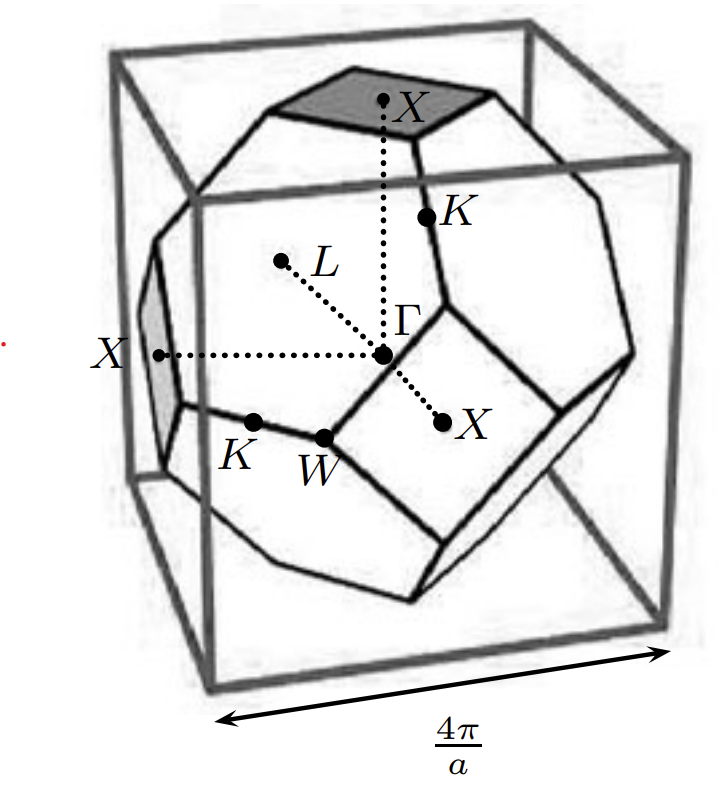
\includegraphics[width=.7\textwidth]{brillouin_zone.png}
        \caption{Brillouinzone}
    \end{figure}
\end{minipage}
\begin{minipage}{0.5\textwidth}
    \begin{figure}[H]
        \centering
        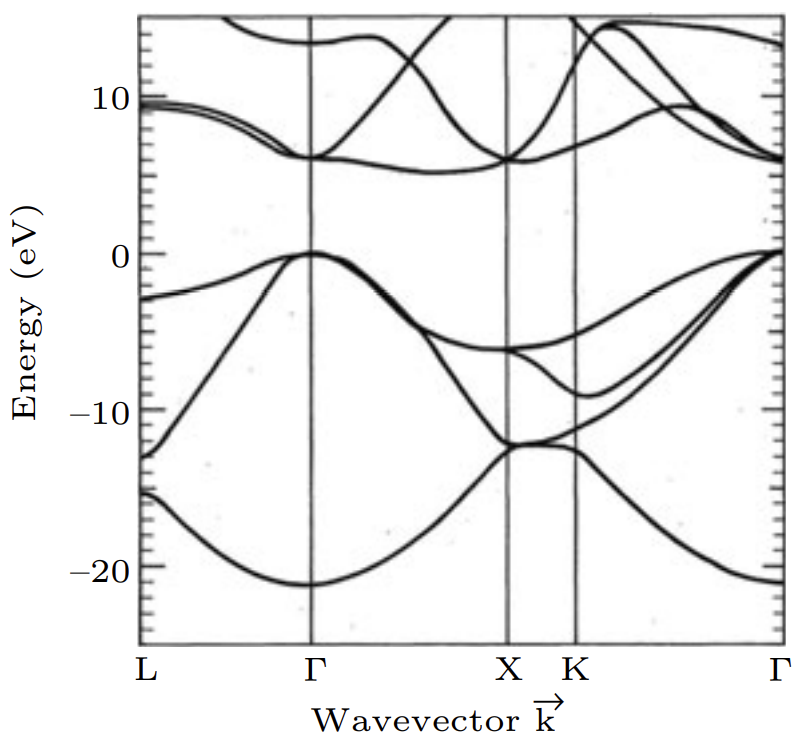
\includegraphics[width=.8\textwidth]{effective_mass.png}
        \caption{Bandstruktur}
    \end{figure}
\end{minipage}


\subsection{Gitterfehler}
Man sortiert Gitterfehler nach ihrere Dimensionalität:
\begin{itemize}
    \item {\bf null} dimensional: Punktefehler, sie sind die einzigen Fehler, die auch im thermischen Equilibrium auftreten, da die Entropie eines Kristalls mit z.B. Leerstellen deutlich höher ist. 
    \begin{enumerate}
        \item {\bf Leerstellen} 
        \item {\bf Zwischengitteratome:} Sitzen auf Plätzen, die im regulären Gitter unbesetzt sind.
        \item {\bf Substitutionsatome:} Sitzen auf Gitterplätzen, die im regulären Gitter durch eine andere Atomart besetzt sind.
    \end{enumerate}
    \item {\bf ein} dimensional: Linienfehler werden gewöhnlich als Versetzungen oder Versetzungslinien bezeichnet. Es gibt Stufen- und Schraubenversetzungen. Beide sind entscheidend für die mechanischen Eigenschaften des Kristalls und daher von großer Bedeutung in den Materialwissenschaften.
    \begin{figure}[H]
        \centering
        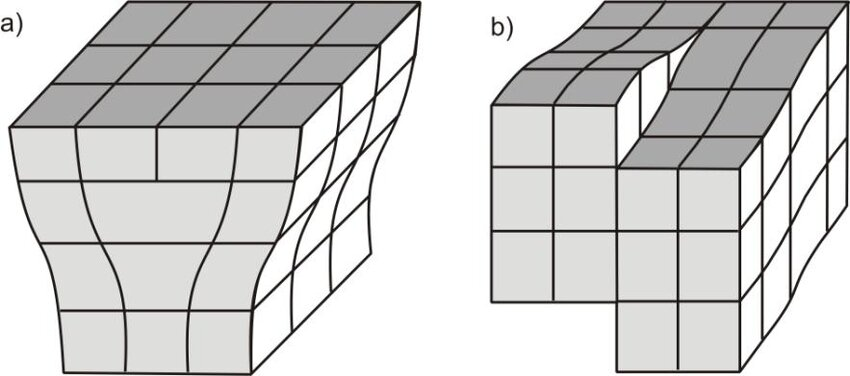
\includegraphics[width=.25\textwidth]{2dfehler.jpg}
        \caption{a) Stufenversetzung, b) Schraubenversetzungen}
    \end{figure}
    \item {\bf zwei} dimensional: Flächenfehler
    \begin{enumerate}
        \item {\bf Oberflächenfehler:} Reale Kristalle haben eine endliche Ausdehnung, die Oberflächen stellen eine Unterbrechung der Translationssymmetrie dar, und damit den einfachsten Flächenfehler.
        \item {\bf Korngrenzen:} Trennen zwei Körner eines Kristalls, d.h. zwei Bereiche mit unterschiedlicher räumlicher Orientierung des Gitters.
        \item {\bf Stapelfehler:} Treten auf, wenn der periodische „Stapel“ der einzelnen Ebenen eines Kristalls gestört ist.
        \begin{figure}[H]
            \centering
            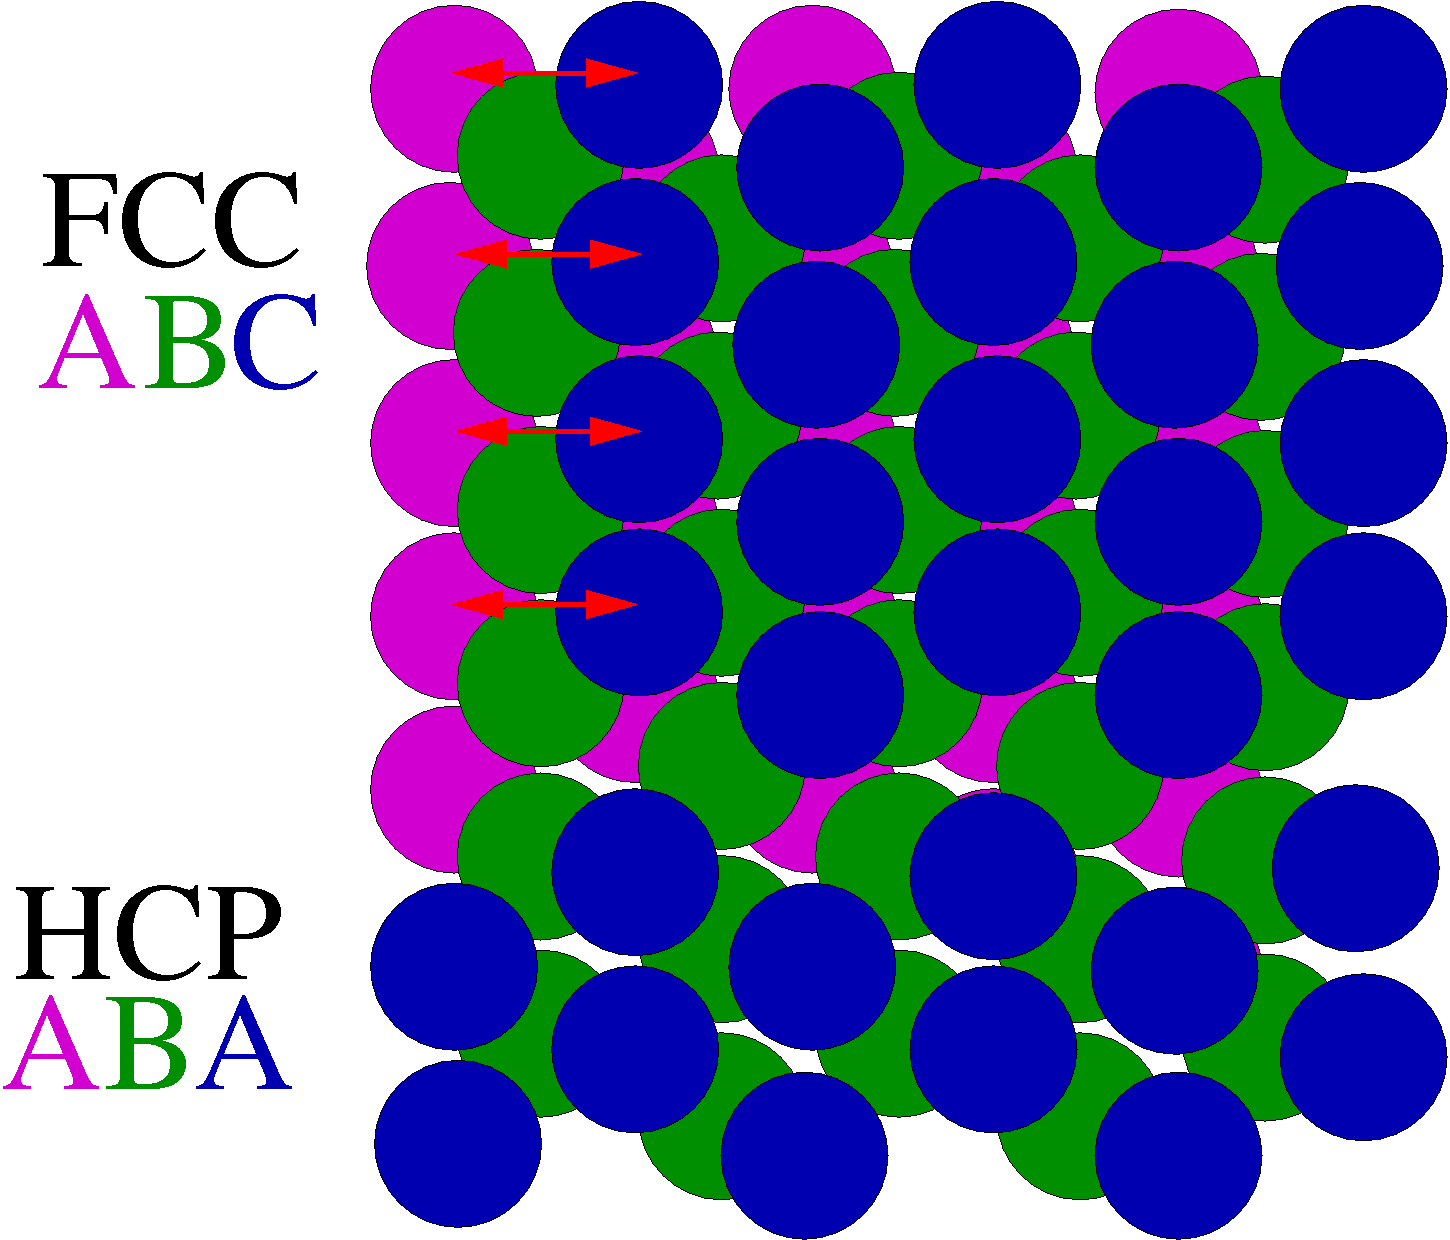
\includegraphics[width=.2\textwidth]{stapelfehler.png}
            \caption{Stapelfehler}
        \end{figure}
        \item {\bf Antiphasengrenze:} Ein Teil des Kristalls ist durch eine Translation gegenüber dem anderen Teil des Kristalls versetzt. Die Translation beträgt nur einen Teil der Gitterkonstante.
    \end{enumerate}
    \item {\bf drei} dimensional: Volumenfehler (auch Inklusionen) sind vollständige Fremdphasen im Inneren des Kristalls. Poren sind offene oder geschlossene Hohlräume im Kristall, die mit Gas oder Flüssigkeit gefüllt sind.
\end{itemize}


\subsection{Beugung und Streuung}
Betrachten wir einen auf einen Kristall einfallenden Strahl mit Wellenvektor $\v k$. Die Übergangsrate nach einem Strahl mit Wellenvektor $\v k'$ ist nach Fermis Goldener Regel gegeben durch 
\begin{align*}
    \fboxed{Fermi's Goldene Regel}{\Gamma(\v k', \v k) &= \frac{2\pi}{\hbar}\sabs{\sbra{\v k'}V\sket{\v k}}^2\delta(E_{\v k}-E_{\v k'})}
\end{align*}
Wir betrachten mit Fermi's Goldener Regel offenbar elastische Streuungen, denn die $\delta$-Funktion lässt nicht zu, dass Energie an den Kristall übertragen wird. Die Existenz bzw. Intensiät  eines Reflex wird durch das Matrixelement $\bra{\v k'} V \ket {\v k} $ bestimmt, welches daher eine zentrale Rolle. Betrachten wir es daher etwas genauer:
\begin{align*}
    \bra{\v k'}V\ket{\v k} &= \iint \dv x' \dv x \sbraket{\v x'}{\v k'}^*\bra{\v x'} V \ket{\v x} \sbraket{\v x}{\v k}
    = \iint \dv x' \dv x \frac{e^{-i \v k' \v x}}{\sqrt{L^3}} V(\v x) \sbraket{\v x'}{\v x} \frac{e^{i\v k \v x}}{\sqrt{L^3}}
    = \frac1{L^3}\int \dv x e^{-i (\v k'-\v k) \v x} V(\v x)
\end{align*}
Es handelt sich bei dem Matrixelemement also um die Fouriertransformierte $\mathscr F_{x\to Q}[V]$ des Potenzials, wobei $\v Q=\v k'-\v k$. Nehmen wir nun an, dass das gesamt Potenzial die Überlagerung des Potenzials einzelner Atome $n(\v x)$ ist.  Die Positionen der Atome werden dabei durch $\delta$-Peaks einer Funktion $A$ dargestellt, sodass man das gesamt Potenzial als Faltung $V(\v x) = A*n$ schreiben kann. Die Positionen der Atome $A$ lassen sich wiederum als Faltung eines Gitter $G$ und einer Basis $B$ darstellen, bzw. mehreren Basen $B_i$, wenn man z.B. ein fcc Gitter in ein sc Gitter mit Basis zerlegt. Damit folgt:
\begin{align*}
    L^3 \bra{\v k'}V\ket{\v k} &= \mathscr F_{x\to Q}[V]
    = \F{G*B_1*\dots B_n} = \F G \F{B_1} \dots \F{B_n}
\end{align*}
Es gibt demnach nur Reflexe, wenn alle Faktoren ungleich null sind. Die Fouriertransformierte von $G$ ist bei allen Kristallen vorhanden und führt deshalb zu einer allgemein anwendbaren Auswahlregel, der sog. Laue-Formel, während die restlichen Faktoren von der spezifischen Form des Kristalls abhängen und dort zu verschiedenen systematischen Abwesenheiten von Reflexen führen. 

Es sei noch erwähnt, dass man die Fouriertransformierte des Potenzials einer PEZ als Strukturfaktor $S_{hkl}$ bezeichnet.

\subsubsection{Laue}
Betrachten wir zunächst den Faktor $\mathscr F_{\v x\to \v Q}[\v G]$, also die Fouriertransformierte des Gitters.
\begin{align*}
    \mathscr F_{\v x\to \v Q}[\v G] &= \sum_{\v G} e^{-i \v Q \v G} \sim \begin{cases}
        \frac{L^3}{V\sub{PEZ}} \for \v Q \v G = 2\pi n\\
        0 \telse 
    \end{cases} = \frac{L^3}{V\sub{PEZ}}\sum_{\v R}\delta_{\v Q,\v R}
\end{align*}
Die Rechnung kann man sich so plausibel machen, dass für $ Q G \neq 2\pi n$ die Potenzialfunktion oszilliert, und im Mittel null ist, während im Fall $Q G =2\pi n$ einfach nur die Elementarzellen gezählt werden. 
Das Ergebnis bedeutet, dass der Kristall nur in Richtungen beugt, bei denen der Impulsübertrag $\v Q = \v k' - \v k$ gerade ein Vektor des reziproken Gitters ist:
\begin{align*}
    \fboxed{Laue-Formel}{\v Q = \v k' - \v k \in R}
\end{align*}

\subsubsection{Bragg}
Eine äquivalente Formulierung der Laue Gleichung ist die bekannte Bragg-Bedingung, man muss nur den Abstand $d$ durch die allgemeine Form des Netzebenenabstandes ersetzen:
\begin{align*}
    \fboxed{Bragg-Bedingung}{n\lambda = 2d_{hkl}\sin\theta = \frac{4\pi}{\abs{\v k^{hkl}\sub{min}}} \sin\theta}
\end{align*}

\subsubsection{Systematische Abwesenheit}
Es kann auch keinen Reflex geben, wenn einer der anderen Faktoren
\begin{align*}
    \F{\v B_n}
    = \sum_{\v B_n}e^{-i\v Q\v B_n}
\end{align*}
verschwindet. Man sagt, dass es für die Kombinationen von h,k,l welche einen Faktor verschinden lassen zur systematischen Abwesenheit kommt.

Beispielweise gilt für einen beliebigen Kristall mit fcc Struktur, welche wir als sc Struktur mit Basis $B=\pug{(000),(\half,\half,0),(\half,0\half),(0,\half,\half)}$ betrachten:
\begin{align*}
    \F{\v B} &= \sum_{\v B}e^{-i\v Q\v B}
    = \sum_{\v B}e^{-i(hb_1 + kb_2 +lb_3)(\alpha a_1+\beta a_2 + \gamma a_3)}
    \overset{(a_i b_j = 2\pi \delta_{ij})}=\sum_{\v B} e^{-2\pi i(\alpha h + \beta k+\gamma l)}\\
    &= 1 + (-1)^{h+k} + (-1)^{h+l} + (-1)^{k+l}
    = \begin{cases}
        4 \for h,k,l \te{ alle gerade oder alle ungerade}\\
        0 \telse
    \end{cases}
\end{align*}
Hier gibt es also unabhängig von der eigentlichen Basis $B_2$ nur Reflexe, wenn $h,k,l$ alle gerade oder alle ungerade sind.

Für die wichtigsten Gitter sind die Auswahlregeln:
\begin{table}[H]
\centering
\begin{tabular}{@{}ll@{}}
    \toprule
    \multicolumn{2}{c}{\bf Systematische Abwesenheiten}\\
    \midrule
    sc & \te{alle $h,k,l$ erlaubt}\\
    bcc & $h+k+l$ \te{ muss gerade sein} \\
    fcc & $h,k,l$ \te{ müssen alle gerade oder alle ungerade sein} \\
    \bottomrule
\end{tabular}
\end{table}

\subsection{Neutronen-Streuung}
Neutronen nur mit den Kernen über die starke Wechselwirkung. 
Das Potenzial eines Atoms ist daher in guter Näherung $V(x) = b \delta(x)$ mit der Streulänge $b$.

\subsection{Röntgen-Streuung}
Photonen Streuung primär an der Elektronenhülle, welche eine nicht vernachlässigbare Ausdehnung hat. Das Potenzial ist daher 
$V(\v x) = f(\v Q)\delta (\v x)$ mit dem Formfaktor $f(\v Q) = \int \dv x e^{i\v Q \v x} n(\v x)$ und der Ladungsdichte $n(\v x)$.

\subsection{Laue Verfahren}
Das Laue-Verfahren wird verwendet um Einkristalle zu untersuchen. Dazu muss
man polychromatische Strahlung verwenden, um mindestens einen erlaubten Bragg-
Reflex zu treffen. In der Ewald-Konstruktion liegen dann zwei Kugeln vor (minimale
und maximale Wellenlänge) zwischen denen dann alle möglichen Reflexe getroffen
werden. Das entstehende Beugungsbild ist ein Punktmuster.

\subsection{Debye-Scherrer-Verfahren}
Das Debye-Scherrer-Verfahren verwendet man zur Untersuchung von Kristalliten. Das angenehm, da es im im Normalfall leichter ist Kristallite zu züchten, als einen homogenen Einkristall. Die Orientierung dieser Kristallite ist zufällig, sodass es immer auch einige gibt, welche die passende Ausrichtung aufweisen, um einen Reflex
zu erzeugen. Daher wird hier monochromatische Strahlung verwendet. Zusätzlich
führt dies dazu, dass das Beugungsbild rotationssymmetrisch ist, also aus Ringen
besteht.

\subsection{Realstruktureffekte}
Es gibt in der Realität einige weitere Effekte, die die Intensität von Reflexen beeinflussen können:
\begin{itemize}
    \item {\bf Multiplizität von Netzebenen:} Verschiedene Netzebenenzahlen können auf $N\sub{hkl}$ verschiedene Arten realisiert werden. Dabei gilt:
    \begin{align*}
        I\sub{hkl}\propto N\sub{hkl} S\sub{hkl}
    \end{align*}
    \item {\bf Gitterschwingungen:} Durch die Anregung von Gitterschwingungen muss ein Korrektur Faktor berücksichtigt werden, der sog. Debye-Waller-Faktor.
    \begin{align*}
        I\sub{hkl}\propto S\sub{hkl} e^{-\alpha^2 G\sub{hkl}^2}
    \end{align*}
    mit dem thermischen Ausdehnungskoeffizienten $\alpha$.
    \item {Endliche Kristallausdehnung:} In vielen Rechnungen sind wir davon ausgegangen, dass das Gitter unendlich ausgedehnt ist. In der Realität ist das natütlich nicht der Fall, wodurch die vorher klaren $\delta$-Reflexe verschmieren. Die Intensität ist annähert proportional zu 
    \begin{align*}
        I\propto N\sub{EZ}^2
    \end{align*}
    der Anzahl an Einnheitszellen.
\end{itemize}

\section{Elektronen im periodischen Potential}

\subsection{Blochtheorem}
Das Blochtheorem sagt aus, dass die Lösungen der Schrödingergleichung in einem periodischen Potential $V(\v x) = V(\v x + \v R)$ gegeben sind durch eine ebene Welle, die durch eine periodische Funktion $u(\v x) = u(\v x + \v R)$ moduliert wird.  
\begin{align}
    \Psi(\v x) &= e^{i\v k \v x} u(\v x)
\end{align}

\subsection{Metalle}
Metalle sind dadurch charakterisiert, dass die Fermienergie ein Band schneidet. Dadurch kann es schon bei Anlegen eines kleinen E-Felds, zu einer Umverteilung der Elektronen (Verschiebung der Fermifläche) hin zu z.B. positiven $\v k$-Wellenvektore, d.h. es fließt ein Strom.

\subsection{Isolatoren }
Isolatoren sind dadurch charakterisiert, dass die Fermienergie in eine (ausreichend große) Bandlücke fällt. Die Elektronen können nicht ohne weiteres Umverteilt werden, und der Material leitet keinen Strom.

\subsection{Halbleiter}
Identisch zu den Isolatoren, jedoch ist die Bandlücke klein, etwa $\sim 1\u{eV}$, sodass durch thermische Anregung Elektronen ins Leitungsband gehoben werden. Sie besitzen also eine mit der Temperatur zunehmende Leitfähigkeit.

Man unterscheided zwischen \emph{intrinsischen Halbleitern} und \emph{Störstellenhalbleitern} (bzw. extrinsischen Leitern), bei denen Elektronen primär durch Dotierung ins Leitungsband gehoben werden.

Weiter unterscheidet man zwischen \emph{direkten} und \emph{indirekten Halbleitern}. Sie unterscheiden sich darin, dass nur beim indirekten Halbleiter ein Elektron beim Übergang ins Leitungsband seinen Impuls bzw. Wellenvektor ändern muss. Im indirekten Halbleiter können Elektronen durch Photonen angeregt werden, beim indirekten Halbleiter nicht, da sie dafür zu wenig Impuls tragen. Der Impuls muss stattdessen von einer Gitterstreuung (Phonon) beigesteuert werden. Bei der Rekombination gilt das Selbe, weshalb sich nur direkte Halbleiter zur Strahlungserzeugung eignen.


\subsection{Metalle, Halbmetalle, Halbleiter und Isolatoren}
Das ausschlaggebene Kriterium zur Kategorisierung nach Metalle, Halbmetalle, Halbleiter und Isolatoren, ist ob die Fermikante der   der Stoffe ein einem Band oder in einer Bandlücke landet.
\begin{figure}[H]
    \centering
    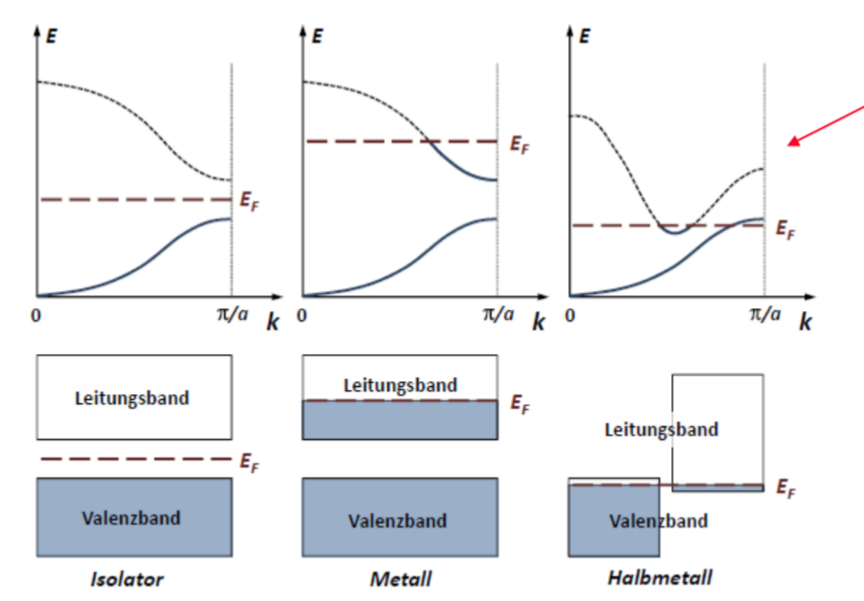
\includegraphics[width=.6\textwidth]{stoffklassen.png}
\end{figure}
Die Eigenschaften von Halbleitern lassen sich durch Dotierung, d.h. das einbringen von Fremdatomen ins Gitter, gezielt verändern. Man unterschiedet zwischen p-Dotierung in die Konzentration der \emph{p}ositiven Ladungsträger erhöht wird, und der n-Dotierung, in der die Konzentration der \emph{n}egativen Ladungsträger erhöht wird. 


\section{Magnetismus}
\subsection{Diamagnetisch}
Diamagnetisch bedeutet, dass die im Material induzierte Dipolfeld \emph{antiparallel} zum anregenden Feld, ist.

\subsection{Paramagnetismus}
Paramagnetismus bedeutet, dass die im Material induzierte Dipolfeld \emph{parallel} zum anregenden Feld, ist. Wichtig dabei ist, dass das Material ohne anregendes Feld keine Dipoldichte hat.
Die magnetische Suszeptibilität des Materials wird durch das Curie-Verhalten charakterisiert:
\begin{align*}
    \fboxed{Curie-Verhalten:}{\chi_m = \frac C T}
\end{align*}

\subsection{Ferromagnetismus}
Identisch zum Paramagnetismus, jedoch sind die Wechselwirkungen im Material so groß, dass es auch ohne externes Feld unter spontaner Symmetriebrechung zur Ausbildung einer Dipoldichte kommt. Oberhalb der Curie-Temperatur $T_C$ geht das Material wieder in einen Paramagneten über und wird im Bereich $T>T_C$ beschrieben durch das Curie-Weiss-Gesetz:
\begin{align*}
    \fboxed{Curie-Weiss-Gesetz}{\chi_m = \frac{C}{T-T_C}}
\end{align*}
mit der Curie-Konstanten $C$.


\section{Supraleitung}

\section{Anhang}
\subsection{Formelzeichen und ihre Bedeutung}
\begin{center}
\begin{tabular}{@{}lll@{}}
    \toprule
    {\bf Formelzeichen} & {\bf Bedeutung} & {\bf Formel} \\
    \midrule
    \(C\) & \(\) & \(\) \\
    \(\beta \) & Kurzschreibweise & \(\frac{1}{k_B T}\) \\
    \(x\) & Kurzschreibweise & \(\frac{\hbar\omega}{k_B T}\) \\
    \(\) & \(\) & \(\) \\
    \bottomrule
\end{tabular}
\end{center}


\end{document}